\documentclass{report}
\title{Billiards}
\usepackage{graphicx}
\usepackage{xfrac}
\usepackage{blindtext}
\usepackage{amsmath}
\usepackage{amsthm}
\usepackage{amsfonts}
\usepackage{mathtools}
\newtheorem{theorem}{Theorem}
\usepackage{titlesec}

\begin{document}

\maketitle
\titleformat{\paragraph}
{\normalfont}{}{}{}
\newpage
\tableofcontents

\chapter{}


\section{The rules of billiard dynamics}
\paragraph{Consider a simple polygonal billiard table, and let a projectile be free to move inside it, similar to a cue ball (Fig 1.1). We assume that all collisions with the sides of the square are completely elastic (i.e., angle of incidence = angle of reflection, and no loss of speed occurs after the collision). We further assume that any collision with a vertex will prevent any further motion (one can imagine that the projectile gets “stuck” at the vertex). \\ \\ }

%Fig 1.1
\begin{center}
\begin{figure} 
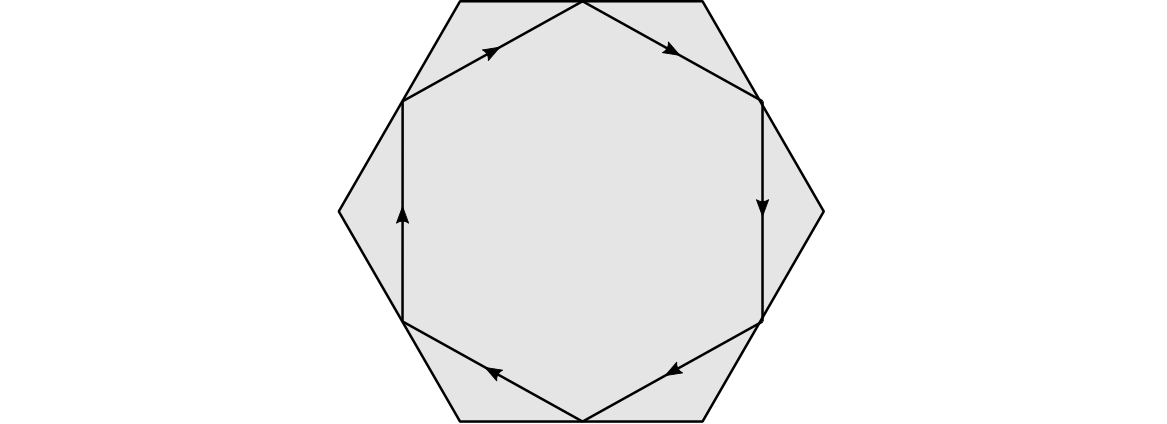
\includegraphics[scale=0.3]{1}
\caption{Trajectory of a cue ball (free particle) on a hexagonal billiard table}
\end{figure}
\end{center}


\paragraph{Note- For reasons that will be clear later, we restrict our discussion to tables in the shape of polygons with an even no of sides, with opposite sides being parallel.}
 
\paragraph{With these rules, we may form possible trajectories inside the table. And these trajectories may be studied using various geometrical manipulations. One powerful method that will be the backbone of our analysis is the idea of identifying edges of a polygon- Given a table of a particular polygon shape, each side can be joined (or “identified”) to its opposite parallel side to create a curved surface (Fig 1.2). This is useful, because it allows us to convert any trajectory into a straight line on that curved surface (Fig 1.3), allowing us to use the geometrical properties of these surfaces to extract information about the trajectories. Note that in the 2D representation of an identified polygon surface, a projectile approaching a side behaves as if it goes into that side, and comes out its identified side (rather like a Pac-man screen)}

\paragraph{Note- It is clear now why we restrict ourselves to polygonal tables with even number of sides- only these shapes can be identified to form a surface.}

%Fig 1.2
\begin{center}
\begin{figure} 
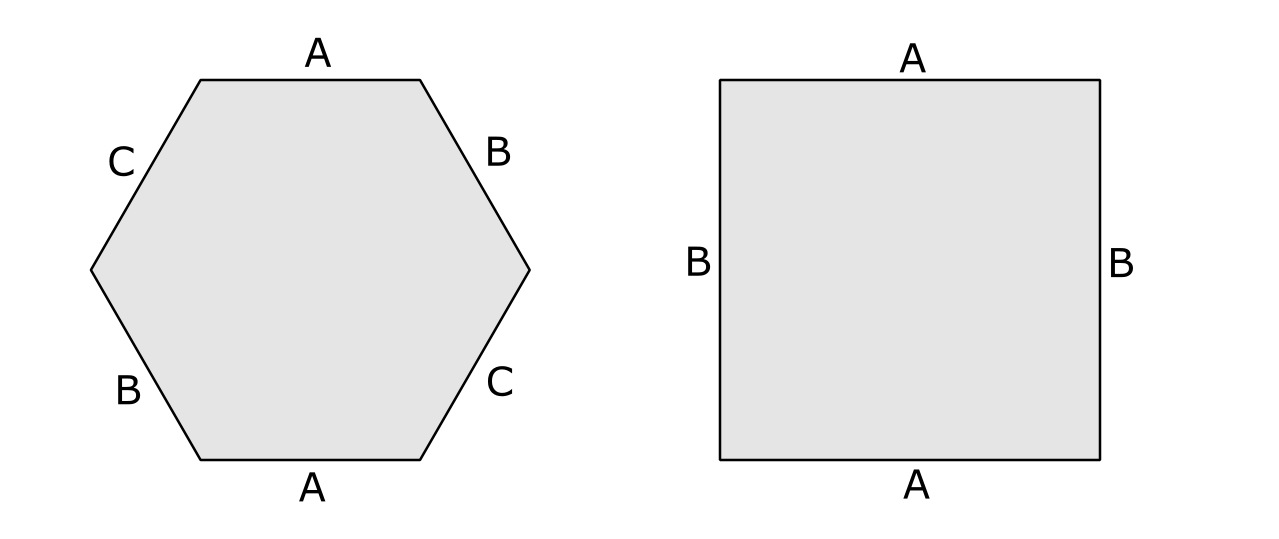
\includegraphics[scale=0.3]{2}
\caption{Polygons with identified edges}
\end{figure}
\end{center}

%Fig 1.3
\begin{center}
\begin{figure} 
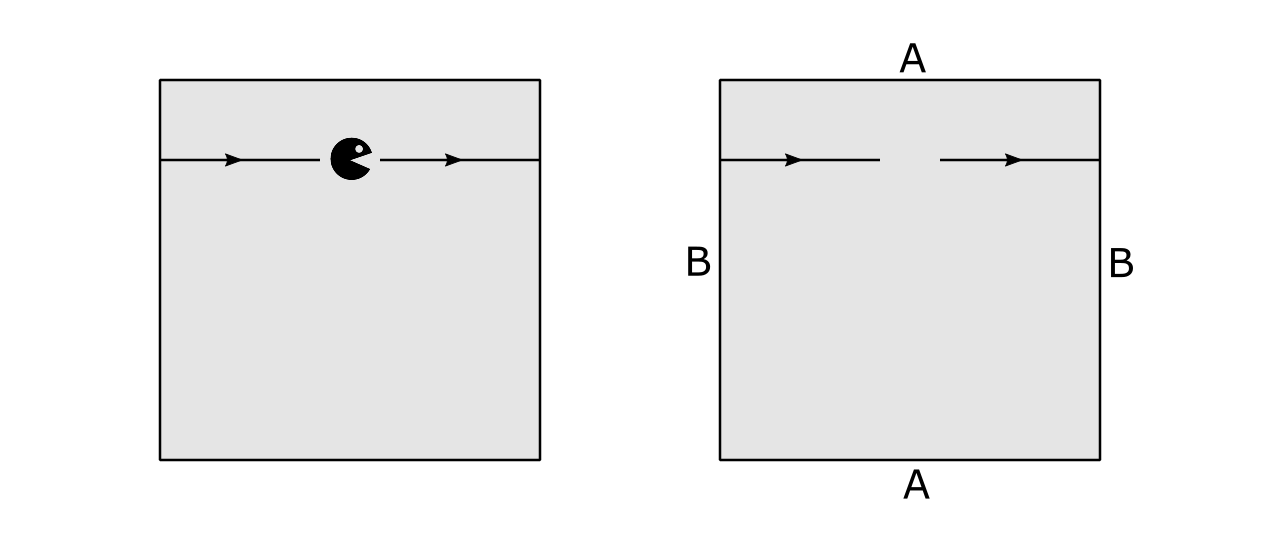
\includegraphics[scale=0.3]{3}
\caption{Comparison between a pac man screen and a trajectory on a polygon identified surface}
\end{figure}
\end{center}

\section{Basic terminology and characterization of trajectories}
\paragraph{Identifying a polygon into a surface results, as one may note, into a continuous representation of the trajectory with a single constant slope at all points. Thus, a trajectory can be uniquely identified by this slope. We will refer to it as \textit{m}}

\paragraph{Given that a projectile moves with slope m then, we would like to be able to keep track of its motion within the polygon. Thus, a method of “bookkeeping” of the projectile’s motion is required to characterize trajectories. One way to do so is by keeping track of which sides the projectile goes through. This is made easy by side identification, since it allows us to treat two identified sides as essentially the same entity.}

\paragraph{We can thus label identified sides uniquely, and create a sequence of all the identified sides that the projectile goes through (Fig 1.4 ). If we write this sequence like a word, then we attain what is known as a cutting sequence. Fig 4 shows some examples}

%Fig 1.4
\begin{center}
\begin{figure} 
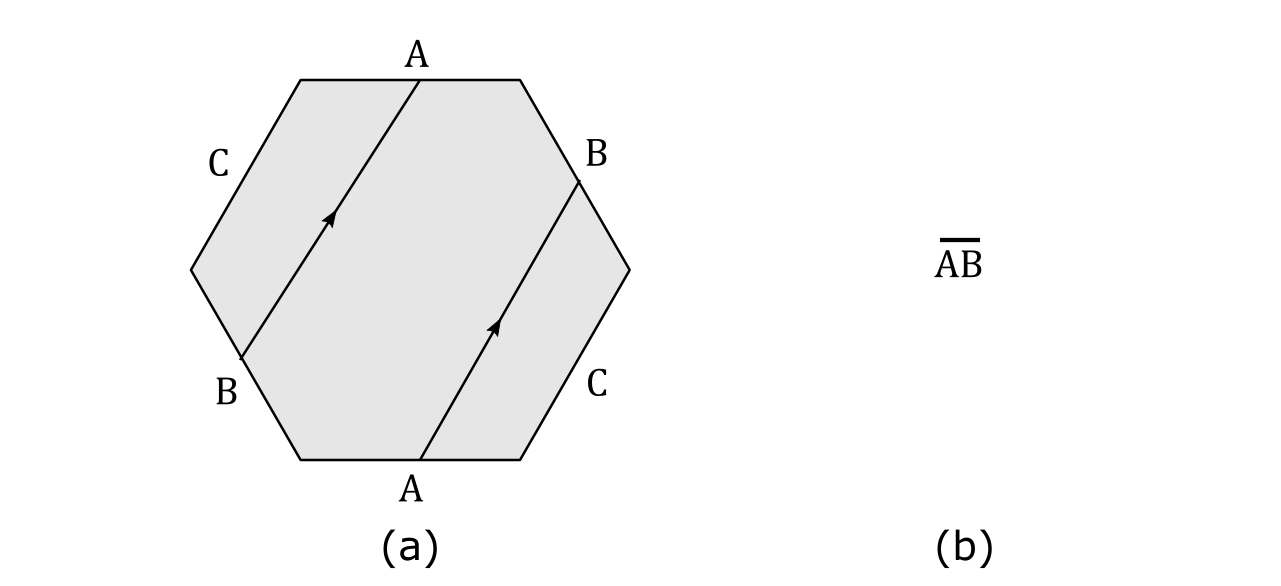
\includegraphics[scale=0.3]{4}
\caption{A trajectory represented (a) graphically and (b) using cutting sequence}
\end{figure}
\end{center}

\paragraph{Describing a trajectory as a cutting sequence, we may try to ask some explicit questions about the trajectory, such as}

\begin{itemize}

\item Given a polygon (and hence the number of labelling letters), which sequences of these letters form a valid cutting sequence?

\item Given a valid cutting sequence, is there any way to use them to determine which trajectories are periodic and which are not?\\ \\ \\

\item Do cutting sequences uniquely represent a single trajectory (does a unique mapping exist between m and a cutting sequence?), or a group of trajectories? And if so, what kind of precise relationship exists between cutting sequences and trajectories?

\end{itemize}

\paragraph{With these basic rules and tools, we now delve into an analysis of these polygon tables geometrically}

\section{The Euler Characteristic $\chi$}

\paragraph{Knowledge of the kind of surface we obtain after identifying a polygon can tell us how to approach the analysis of billiard dynamics on it. We may try to predict the obtained surface by tricky geometrical manipulations and visualization, or we may use the concept of the Euler Characteristic.}

\paragraph{We define Euler Characteristic as follows}

\paragraph{\textit{DEFINITION:} Given a surface \textit{S} made by identifying edges of polygons, with \textit{V} vertices, \textit{E} edges, and \textit{F} faces, its Euler characteristic $\chi$ is}

\begin{equation}
\mathit{\chi(S)=V-E+F}
\end{equation}

\paragraph{In topology, the genus (the number of “holes” in a surface) of the surface plays an important role. From classification of the surfaces to developing homeomorphism between two surfaces, we need to know the genus of the surface.}

\paragraph{The following theorem is an explicit relationship between Euler’s characteristic and the genus of an orientable surface (any surface with a well defined orientation):}

\paragraph{\textit{THEOREM}: A surface \textit{S} with genus \textit{g} has Euler characteristic given by}

\begin{equation}
\chi=2-2g
\end{equation}

\paragraph{We use these numbers to identify a surface uniquely. If two polygons can both be identified into a common surface with a particular Euler Characteristic $\chi$, then the dynamics for both polygons are the same (since in the surface, the dynamics end up being the same). Since the Euler characteristic can be calculated from just knowledge of the polygon, we can figure out which surface a polygon can form without any complex visualizations.}

\paragraph{In order to apply the Euler characteristic to our use, we must know vertices, edges and faces of the polygon. For a given polygon with identified edges, we can find edges and faces of the polygon without much effort.}

\paragraph{To count the vertices, we implement the following sequence of steps:}


\begin{enumerate}

\item Pick a side 1, it has an identified side 1’. Pick a vertex on 1. It has an identified vertex on 1’.

\item The chosen vertex on side 1 is connected to another side (call it 2. The side 2’, identified to 2 is connected to 1’ in the same sense (clockwise or anti-clockwise) as 2 is to 1.

\item Since 2 has the chosen vertex, the corresponding vertex on 2’ can be identified to the two vertices already identified in step 1.

\item Continue this process till we reach the original polygon vertex from step 1. At this point, choose any unidentified vertices, and repeat the process.

\end{enumerate}


\paragraph{We iterate this process repeatedly till we have covered every polygon vertex (Note that the number of iterations = the number of surface vertices)}

\paragraph{Figure (1.5) illustrates vertex counting scenario for a hexagon}

%Fig 1.5
\begin{figure} 
\begin{center}
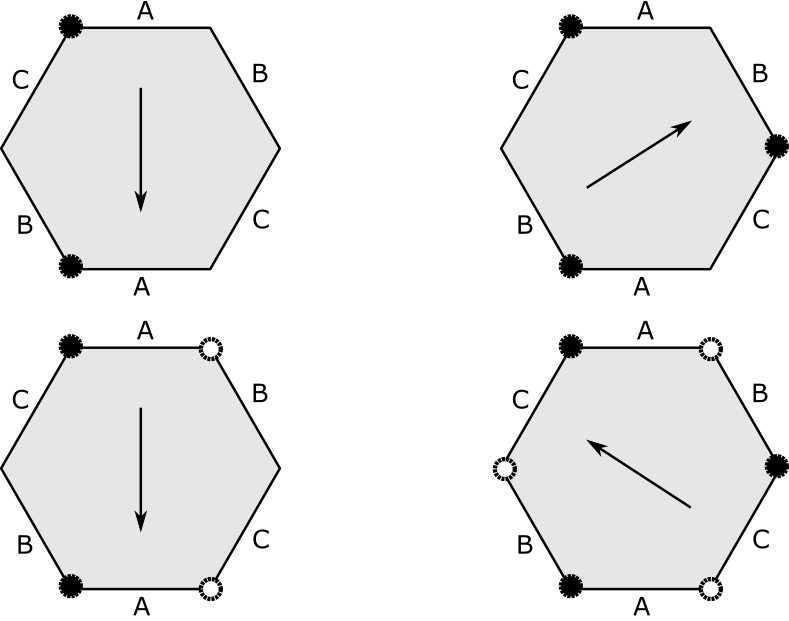
\includegraphics[scale=0.3]{5}
\caption{An identified hexagon has 2 vertices}
\end{center}
\end{figure}

\paragraph{A number of theorems can be proven regarding the number of vertices in a polygon identified surface. We illustrate a few of them in the appendix}


\section{Symmetries and transformations}

\paragraph{Symmetries of a polygon are linear bijective transformations which map between points in the same space such that vertices of a polygon are mapped back to vertices (a vertex may be mapped to a different one). 
These symmetries are of interest because, among other reasons, a symmetric transformation of the polygon, applied to a valid trajectory on that polygon, gives us another valid trajectory.}

\begin{enumerate}

\item Reflection along x
$ (\begin{bmatrix}
1&0\\0&-1
\end{bmatrix})$
or y
$ (\begin{bmatrix}
-1&0\\0&1
\end{bmatrix})$

\item Rotation by $\pi/2$ radians
$ (\begin{bmatrix}
0&-1\\1&0
\end{bmatrix})$

\item Shearing

%Fig 1.6
\begin{figure} 
\begin{center}
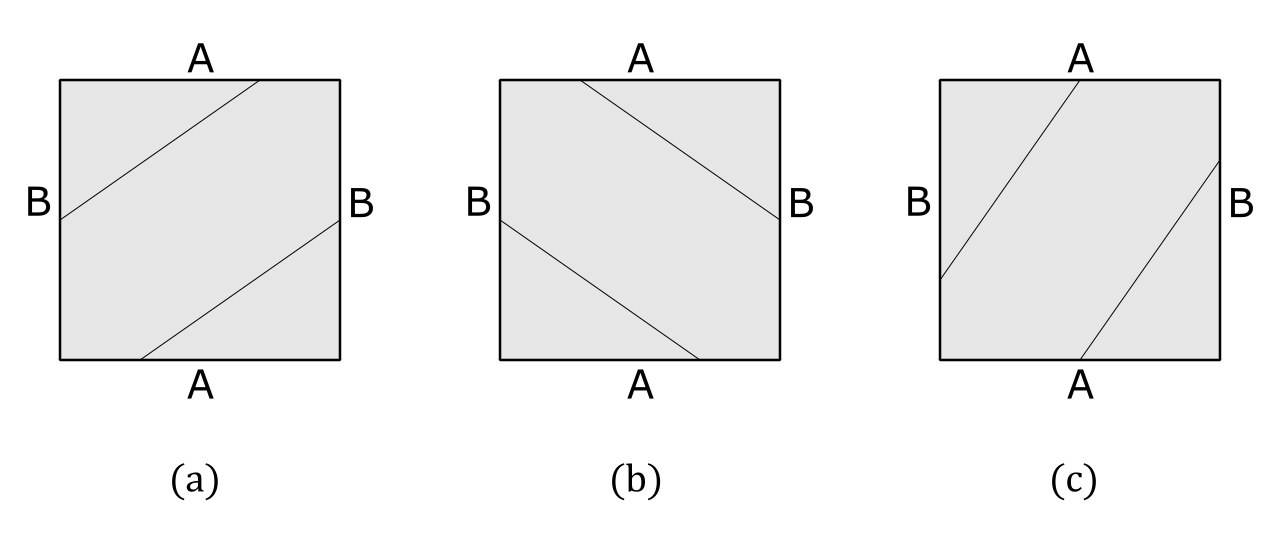
\includegraphics[scale=0.3]{6}
\caption{Trajectory of slope 7/10 and (b) the result of a horizontal or vertical reflection, (c) reflection along a positive and negative diagonal}
\end{center}
\end{figure}

%Fig 1.7
\begin{figure} 
\begin{center}
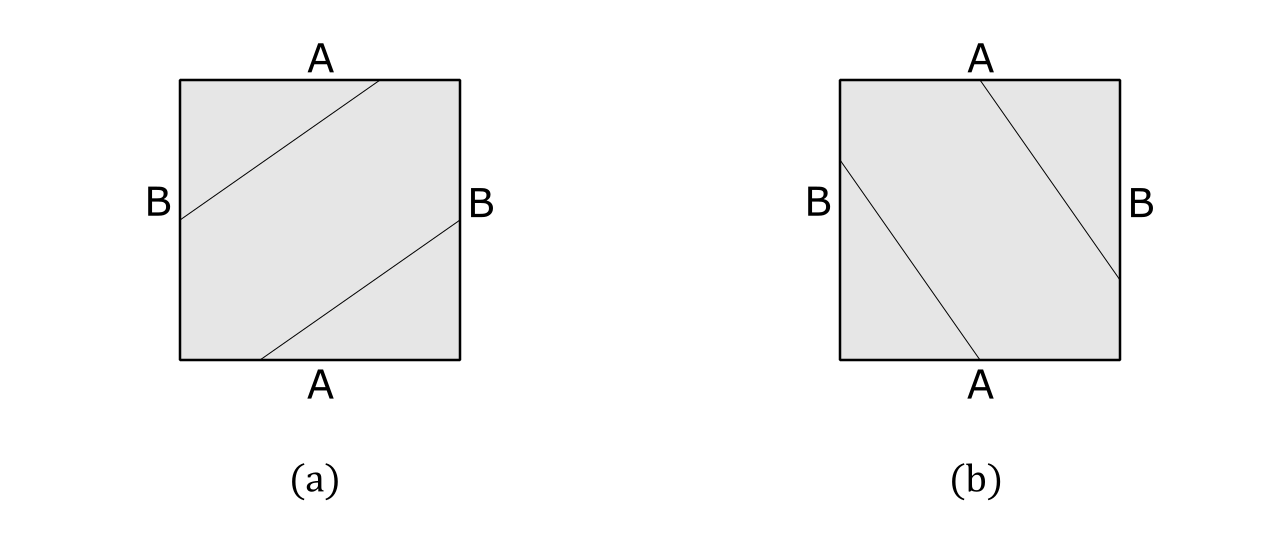
\includegraphics[scale=0.3]{7}
\caption{Trajectory of slope 7/10 and (b) the result of a $\pi$/2 clockwise or anticlockwise rotation}
\end{center}
\end{figure}

\end{enumerate}


\paragraph{Among these, shearing requires a bit more careful study.}



\section{Shears and one directional scaling}


\paragraph{When a surface is twisted in a direction such that points on a line parallel to this direction remain stationary, we call it shearing of the surface. (Fig 1.8)}

%Fig 1.8
\begin{figure} 
\begin{center}
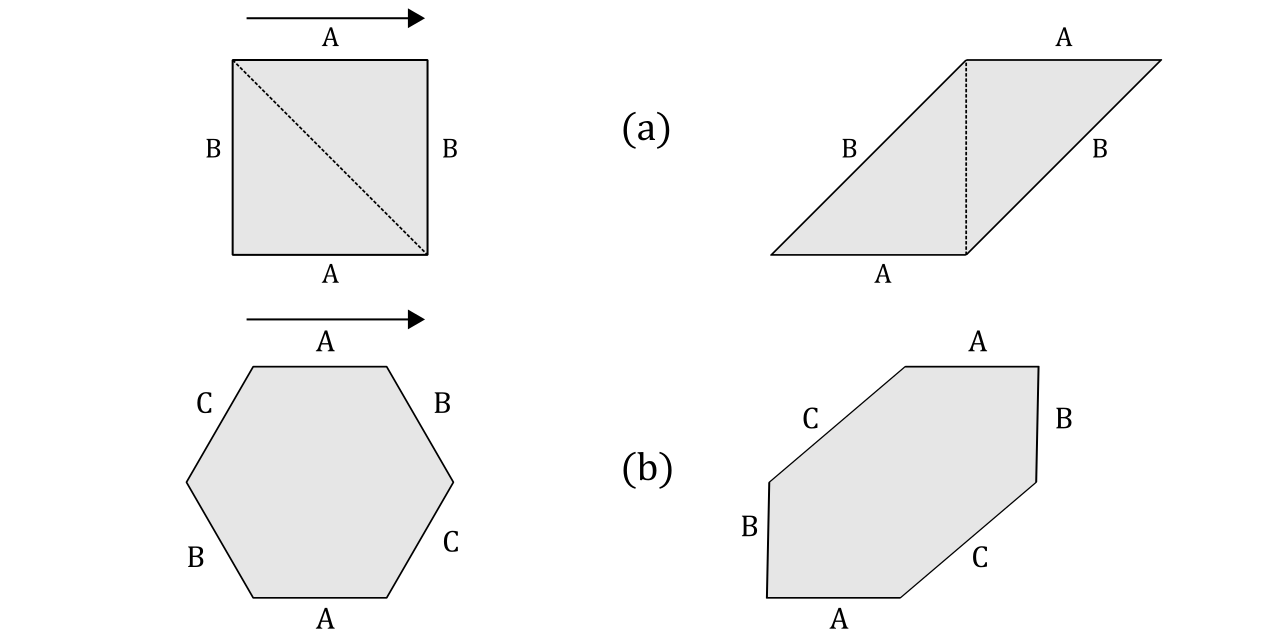
\includegraphics[scale=0.3]{8}
\caption{Shearing (a) a square torus and (b) a hexagon horizontally}
\end{center}
\end{figure}


\paragraph{\textit{DEFINITION}: A linear transformation of the form
$ (\begin{bmatrix}
1&m\\0&1
\end{bmatrix})$
or
$ (\begin{bmatrix}
1&0\\m&1
\end{bmatrix})$
where m is any integer, is a one directional shear map.
}

\paragraph{There are two types of shear maps:}

\begin{itemize}
\item Horizontal shear mapping takes a point on the surface (x,y) and transforms it to (x+my,y), where m is a fixed constant known as shear factor. Such a shear is also known as shear parallel to x-axis. It is represented by 
$ (\begin{bmatrix}
1&m\\0&1
\end{bmatrix})$ 

\item Vertical shear mapping takes a point on the surface (x,y) and transforms it to (x,mx+y), where m is a fixed constant known as shear factor. Such a shear is also known as shear parallel to y-axis. It is represented by
$ (\begin{bmatrix}
1&0\\m&1
\end{bmatrix})$ 
\end{itemize}

\paragraph{We must not confuse shearing with rotation. Shearing distorts the 2D shape of the surface. If we rotate a square, we will always get a square in 2D.}

\paragraph{Note that shearing preserves properties like parallelism and area. It also preserves the side identifications of the polygon (since parallel sides remain parallel to each other after shearing). Thus, shearing a polygon does not change the 3D surface it is identified into.}

\paragraph{We will usually cut the sheared polygon and rearrange the individual pieces (while respecting side identifications) to retrieve the original polygon shape for ease of analysis.}

\paragraph{Shearing can be observed in both 2D and 3D spaces. For studying billiards, we will restrict ourselves to 2D shearing maps.}



\section{Periodicity of trajectories}

\paragraph{Identifying sides of a polygon to create a surface in 3D gives us (as we have discussed) a way to represent a trajectory on the polygon in terms of a continuous line, with a single well defined slope in the flat plane. There is another (and essentially similar) way of representing this trajectory, as follows:}

%Fig 1.9
\begin{figure} 
\begin{center}
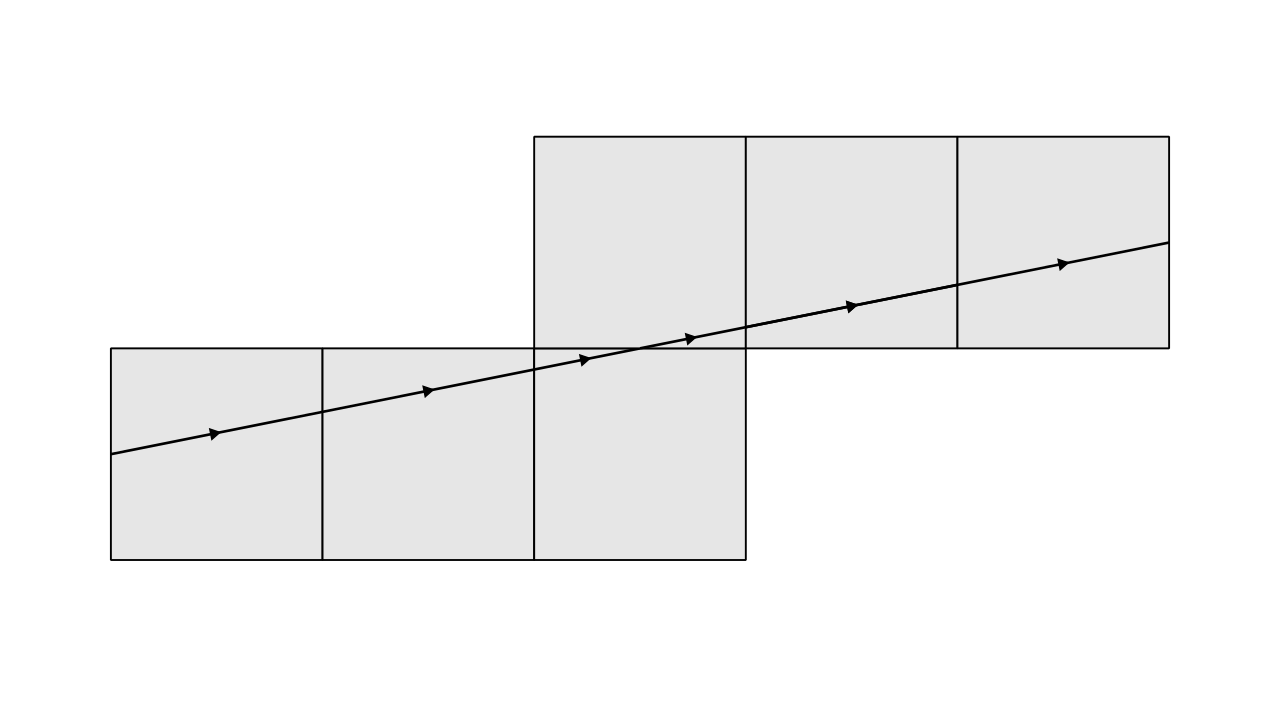
\includegraphics[scale=0.3]{9}
\caption{Unfolding a trajectory on a square torus}
\end{center}
\end{figure}

\paragraph{We assume the projectile on the table starts off in a particular direction (say, angle $\theta$ and slope $m = tan\theta$). When it hits a particular side, we simply create a mirror reflection of the polygon about that side (“unfold” the table in the direction of that side), and let the projectile continue on its path in the same direction. Every time it hits a side, we unfold the polygon along that side (Fig 1.9).\\ \\ \\ \\ \\}

\pagebreak

\paragraph{The result is that we get a tiled representation of the flat plane (a graph, of sorts) on which the trajectory is a straight line of slope $m$. We call this the unfolded trajectory.}



\paragraph{We introduce this method because it enables us to easily determine which trajectories in a polygonal table are periodic, and which are not.}

%Fig 1.10
\begin{figure} 
\begin{center}
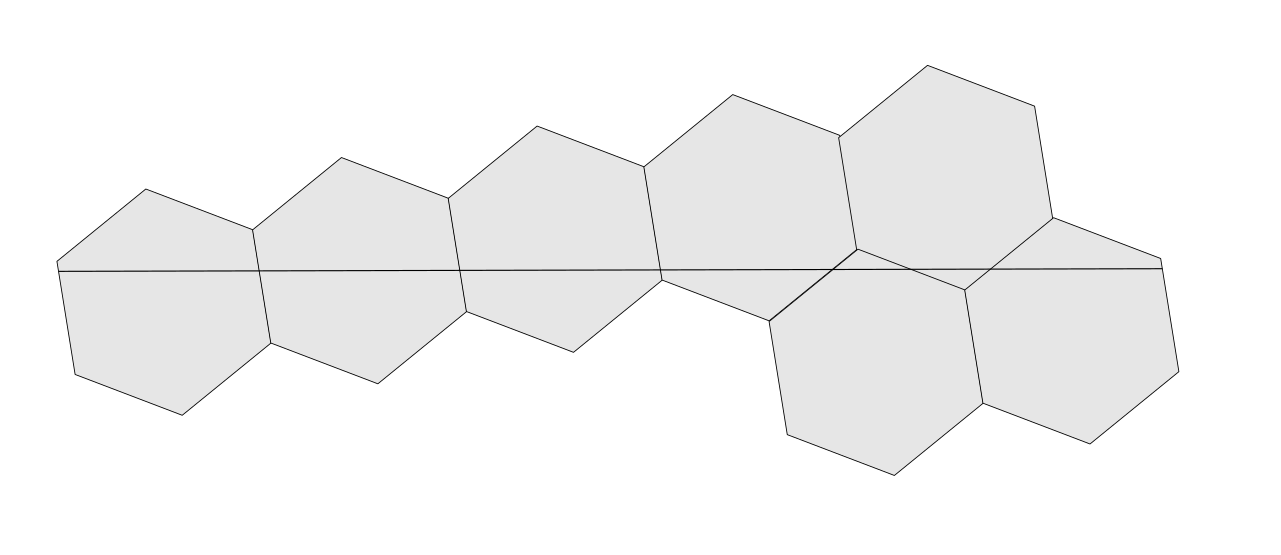
\includegraphics[scale=0.3]{10}
\caption{Periodic trajectory (unfolded) on a hexagon}
\end{center}
\end{figure}

\paragraph{If a trajectory of slope $m$ would be periodic on a particular polygon table, then it means that on the unfolded trajectory, it will pass through the same point on a different polygon as it started from in the first polygon (i.e, it joins corresponding points on two separate polygons on the tiled representation) (Fig 1.10). Conversely, if the trajectory passes through a point on the $n$th polygon that corresponds to the starting position of the first polygon, then the trajectory is periodic. Thus, we know that passing through the same position as the starting position on the $n$th polygon is a sufficient and necessary condition for periodicity. Moreover, the period of the trajectory is $n$.}

\paragraph{To completely describe such trajectories, we will first create a special periodic trajectory, and use it to create more general ones.}

\paragraph{Consider a polygonal billiard table, and the unfolded tiled representation of the table. Consider a trajectory that starts at the center of the first polygon, and passes through the center of the $n$th polygon that it crosses. Clearly, it is a periodic trajectory of period $n$. Let its slope be $m$.}

%Fig 1.11
\begin{figure} 
\begin{center}
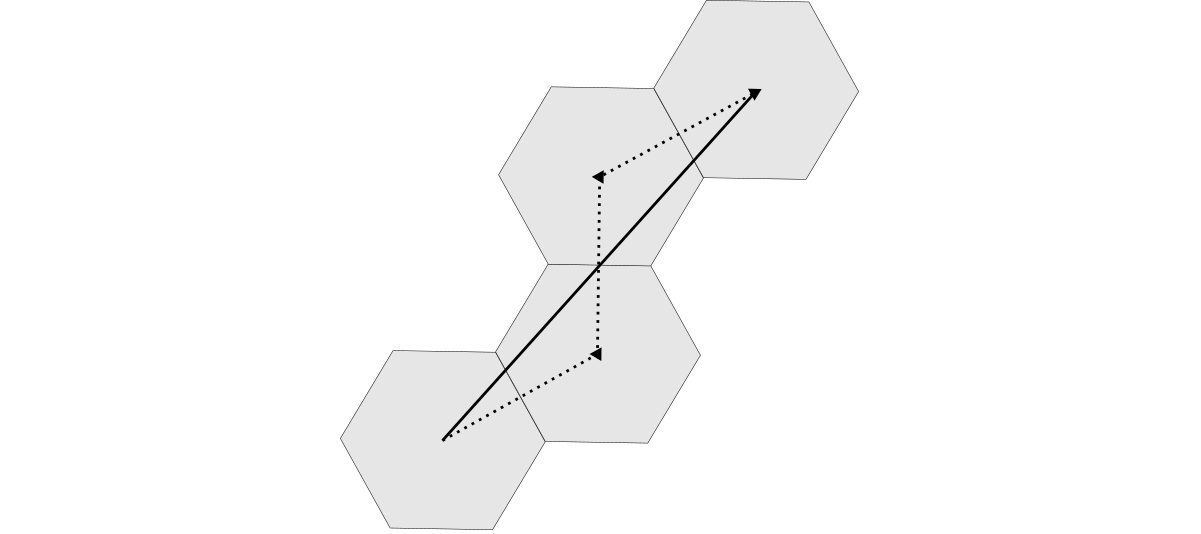
\includegraphics[scale=0.3]{11}
\caption{Center to center decomposition of a center to center trajectory}
\end{center}
\end{figure}

\paragraph{We can create a reconstruction of this trajectory by first creating an ordered sequence of all the polygons that the trajectory passes through, and then joining the centers of the adjacent polygons in the sequence (An illustration of this is shown in (Fig 1.11)). \pagebreak This is a vector decomposition of the trajectory, where each of the constituent vectors are of equal length, and their directions correspond to the normal to each of the sides of the polygon in question. This set of vectors for each polygon can thus be used to construct a center to center trajectory. Call this set $E$.}

\paragraph{We can generalize this by noting that a center to center trajectory can be translated in such a way that it connects any two corresponding points of the $1$st and $n$th polygon, with the same vector decomposition as before (since all vectors stay constant under a translation), as well as the same slope (Fig 1.12). Since we have already seen that the general periodic trajectory always connects corresponding points of two polygons in the tiled representation, we can see that the vectors used to construct a center to center trajectory of slope $m$ can be used to construct any periodic trajectory of slope $m$ (i.e, a trajectory of slope $m$ with any starting point, or simply, the general trajectory of slope $m$).}



%Fig 1.12
\begin{figure}
\begin{center}
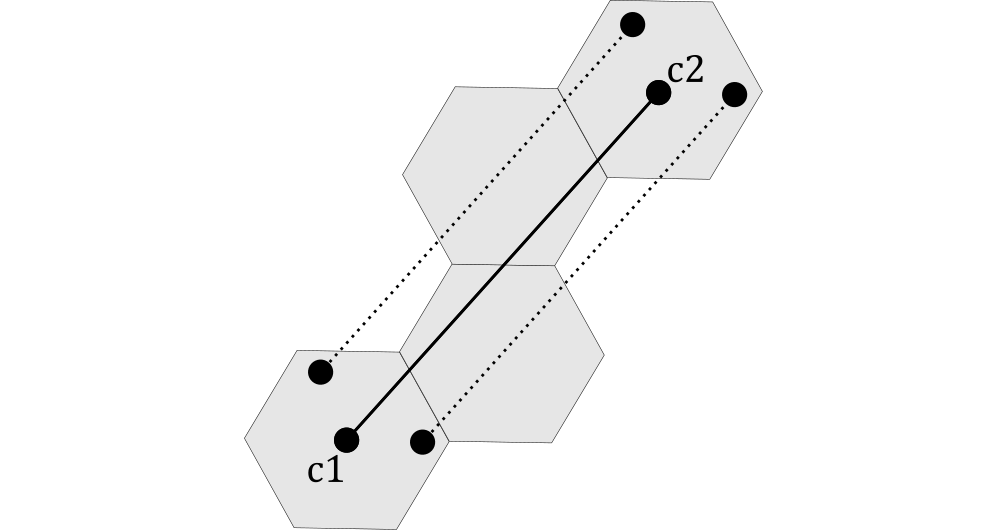
\includegraphics[scale=0.3]{12}
\caption{Translating a center to center trajectory can help us describe all periodic trajectories of the same slope}
\end{center}
\end{figure}


\paragraph{There is hence a very powerful relationship between the nature of the polygon, and the periodicity conditions of a trajectory on it. This can be encapsulated in the following theorem:}

\pagebreak

\paragraph{$THEOREM$- For a given polygon $P$, let $E_P = {e_1,...e_k}$ be the set of the normal vectors to the sides of the polygon (all of the same length). Then any periodic trajectory on the polygon can be constructed by an integer combination of the vectors in $E_P$. Moreover, the slope for a periodic trajectory is necessarily given by.}

\begin{equation}
m=\frac{\sum_{i=1}^k  c_ie_{yi} }{\sum_{i=1}^k  c_ie_{xi} }  
\end{equation}

\paragraph{where $c_i \in \mathbb{N}$, and $e_{xi}, e_{yi}$ are the $x$ and $y$ components respectively of the $ith$ vector in $E_P$}

\paragraph{\textit{Proof}:~We have already seen how the vectors of $E_P$ can construct any periodic trajectory. Suppose a particular periodic trajectory of slope $m$ and period $n$ can be decomposed as follows:}

\begin{equation}
\vec{\tau}=\sum_{i=1}^k c_ie_i 
\end{equation}

\paragraph{where $\vec{\tau}$ is a vector starting at the first polygon, ending at the $nth$ polygon (basically a vector representation of the trajectory) and all $c_i$ are integers}

\paragraph{If we consider the starting point of $\vec{\tau}$ as the origin, then the slope $m$ is just $\frac{y}{x}$, where $x$ and $y$ are the coordinates of (we can do this because the vector decomposition remains the same irrespective of the origin). From the vector addition laws, it is clear that $x$ and $y$ are given by}

\begin{equation}
y=\sum_{i=1}^k c_ie_{yi}\quad and
\quad x=\sum_{i=1}^k c_ie_{xi}
\end{equation}

\paragraph{where $e_{xi}, e_{yi}$ are the $x$ and $y$ components respectively of the $ith$ vector in $E_P$. $m$ is thus given by:}

\begin{equation}
m=\frac{\sum_{i=1}^k  c_ie_{yi} }{\sum_{i=1}^k  c_ie_{xi} }
\end{equation}

\paragraph{The numbers $c_i$ have an important interpretation- they represent the number of times we apply $e_i$ in the construction of a particular trajectory. Since $e_i$ is the normal vector of a unique side of the polygonal table in question, and since the unfolded trajectory treats each side of the $nth$ polygon the same as the corresponding opposite side in the $n+1th$ polygon in the tiled representation (similar to the identification process), we say that $c_i$ represents the number of times a trajectory passes through the side with normal vector $e_i$ on the identified table.}

\paragraph{Note- The period n of the trajectory is given by $\sum_{i=1}^k c_i$ , since $n$ is the number of polygons that the trajectory goes through in the tiled representation before it repeats itself, and each $c_i$ is the number of times the $ith$ vector in $i$ is applied. Thus, $\sum_{i=1}^k c_i$ is the total number of times a vector from $E$ is applied. Since a vector from $E$ is applied each time the trajectory enters a new polygon in the tiled representation, we find that $n = \sum_{i=1}^k c_i$
}

\paragraph{We end this section by analyzing periodicity in a square table:}

\paragraph{Periodicity in a square table- Unfolding a square table is a particularly interesting procedure, for it gives us a square grid (essentially a rectangular coordinate system). This makes our analysis simple; for any particular square in the grid, the normal vectors are horizontal and vertical. Since the choice of length is arbitrary (we only need the length to be uniformly equal), we choose unit length (assuming that the side of the square is taken as the unit length)}

\paragraph{Thus, for a square, we can write E = \{$\hat{i},\hat{j}$\}, where $\hat{i}$ and $\hat{j}$ are the unit coordinate vectors. In a square table, then, any periodic trajectory is one that can be written as an integer combination of $\hat{i}$ and $\hat{j}$.}

\paragraph{From the equation for m derived previously for the general polygon, we get}

\begin{equation}
m=\frac{\sum_{i=1}^k  c_ie_{yi} }{\sum_{i=1}^k  c_ie_{xi} }=\frac{(c_1)(0)+(c_2)(1)}{(c_1)(1)+(c_2)(0)}=\frac{c_2}{c_1}
\end{equation}

\paragraph{where $c_2$ and $c_1$ are the number of times the trajectory passes through the horizontal and vertical sides of the squares on the identified square.}

\paragraph{We see that $m$ is necessarily a rational number. Thus, periodic trajectories on a square table correspond to rational slopes. Also, we see that the period $n$ is given by $n = c_1 + c_2$}






\chapter{Billiard dynamics on the square torus}

\paragraph{In this chapter, we take the example of a simple polygon- the square- and describe billiard dynamics in it. A square has an even number of sides, with opposite sides being parallel. Thus, we can use all the tools and methods that we introduced in chapter 1, and we will see they give us a very good description of the general trajectory on a square table, owing to the specific properties of the square.}

\section{The Square torus and identifying sides}

\paragraph{If we identify the opposite sides of a square, we obtain a 3D object called a torus. A square torus in a 2D plane looks exactly like a flat square but has only two distinct sides, A and B, each of which is represented by a set of opposite sides on the flat square (Fig 2.1) A square torus has a genus of 1, and Euler Characteristic value of 0 (calculated as per the formulae given in Ch 1).}

%Fig 2.1
\begin{figure}[h]
\begin{center}
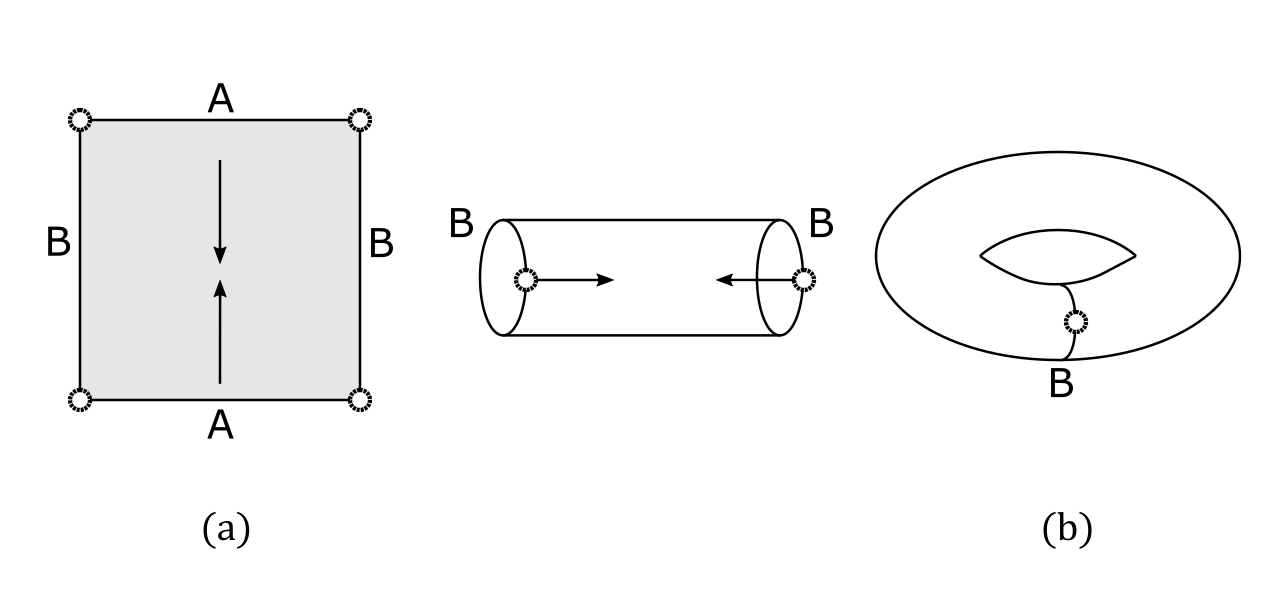
\includegraphics[scale=0.3]{2.1}
\caption{(a) Glueing identified sides of a square to form a square torus (b) A torus in 3 dimensions}
\end{center}
\end{figure}

\pagebreak


\paragraph{Note: We make a distinction between a square torus and  torus. A square torus is simply a 2D representation of a torus in terms of a square. We may make a parallelogram torus in this way too, for example (Fig 2.2)}

\paragraph{Notice that a square torus has one surface vertex (Fig 2.3). Also, the angle around the vertex is $4\frac{\pi}{2} = 2\pi$, making the vertex indistinguishable from any other point on the surface (i.e, a flat surface).}


%Fig 2.2
\begin{figure}[h] 
\begin{center}
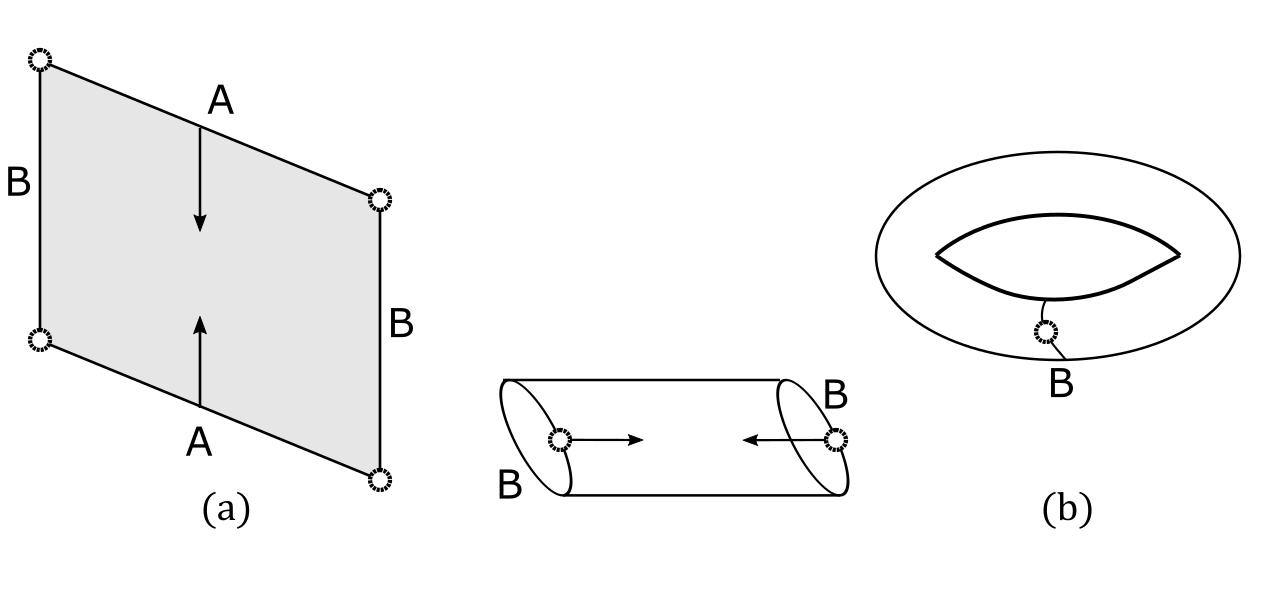
\includegraphics[scale=0.3]{2.2}
\caption{(a) Glueing identified sides of a parallelogram to form a parallelogram torus. (b) The torus formed in the process (same as that from a square)}
\end{center}
\end{figure}


\section{Cutting sequences on a Square Torus}


%Fig 2.3
\begin{figure} 
\begin{center}
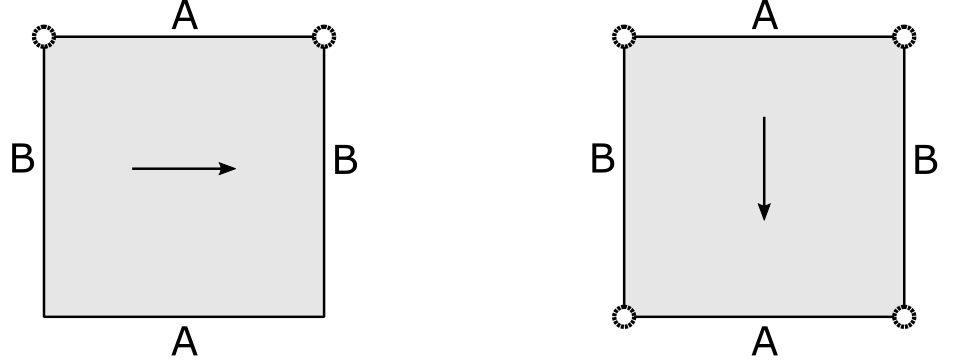
\includegraphics[scale=0.3]{2.3}
\caption{ A square torus has 1 surface vertex}
\end{center}
\end{figure}


\paragraph{Trajectories on a square torus can be described, like any other identified polygon, in terms of cutting sequences. For a square torus, since we have only two distinct sides A and B, the cutting sequences are bi-infinite permutations of A’s and B’s (Fig 2.4). For periodic trajectories, note that the cutting sequence will be a finite permutation repeated infinitely.}



\paragraph{In Chapter 1, we stated an equation to find the slope of a trajectory on the square table.}


\begin{displaymath}
{M_{(slope)}=\frac{c_{2}}{c_{1}}}
\end{displaymath}


\pagebreak

\paragraph{where $c_{2}$ and $c_{1}$ are the number of times the trajectory passes through the horizontal and vertical sides respectively on the identified square.\\ Since we have labelled the horizontal identified side as A, and the vertical identified side as B, we can state the following:}


\paragraph{\textit{Theorem}: For a cutting sequence given by a finite number of A’s and B’s (i.e, a periodic trajectory), we can determine the slope of the trajectory by the following relation:}

\begin{equation}
{Slope = \frac{\text{\# of A's in the cutting sequence}}{\text{\# of B's in the cutting sequence}} }
\end{equation}


\paragraph{(proof in appendix) 
(appendix also has a section on drawing trajectories given the cutting sequences, with example exercises and proof of Ex 3.3)}

\paragraph{Finding the slope from the cutting sequence seems quite easy, but the reverse is a more involved process. This will be introduced later in the chapter, giving us a complete relationship between slope and cutting sequence of a trajectory.}


%Fig 2.4
\begin{figure} 
\begin{center}
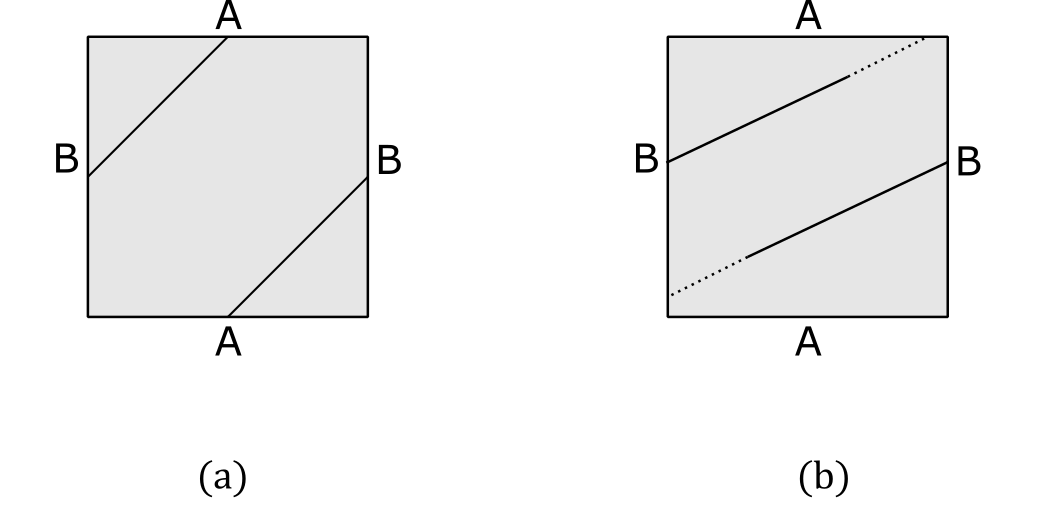
\includegraphics[scale=0.3]{2.4}
\caption{(a) Periodic trajectory $\overline{AB}$ (b) A non periodic trajectory given by ...BBA... (only part of the trajectory is shown)}
\end{center}
\end{figure}

\pagebreak

\section{Symmetries of the square torus}

\paragraph{For a square, we have the usual polygon symmetries corresponding to rotation and reflection, and the usual defined shear map.}

\paragraph{We have the following specific symmetries available for the square:}

\begin{enumerate}
\item  {\emph{Reflection:}With a fixed vertex we can observe the reflection symmetry of a square torus along vertical, horizontal and diagonal lines of symmetry.(Fig 2.5) }


\item  {\emph{Rotation:}We can observe rotation symmetry by rotating the square torus by a multiple of $\pi/2$. (Fig 2.6 and Fig 2.7)}

\item  {\emph{Shear:}As defined before (Fig 2.8). \\  \\ Note that a shear map on the square does not necessarily map it back to a square (since interior angles are not respected by shear maps, they map to a parallelogram in general). The necessary rearrangement involves translating a part of the parallelogram as shown in the figure. }

\end{enumerate}


%Fig 2.5
\begin{figure} 
\begin{center}
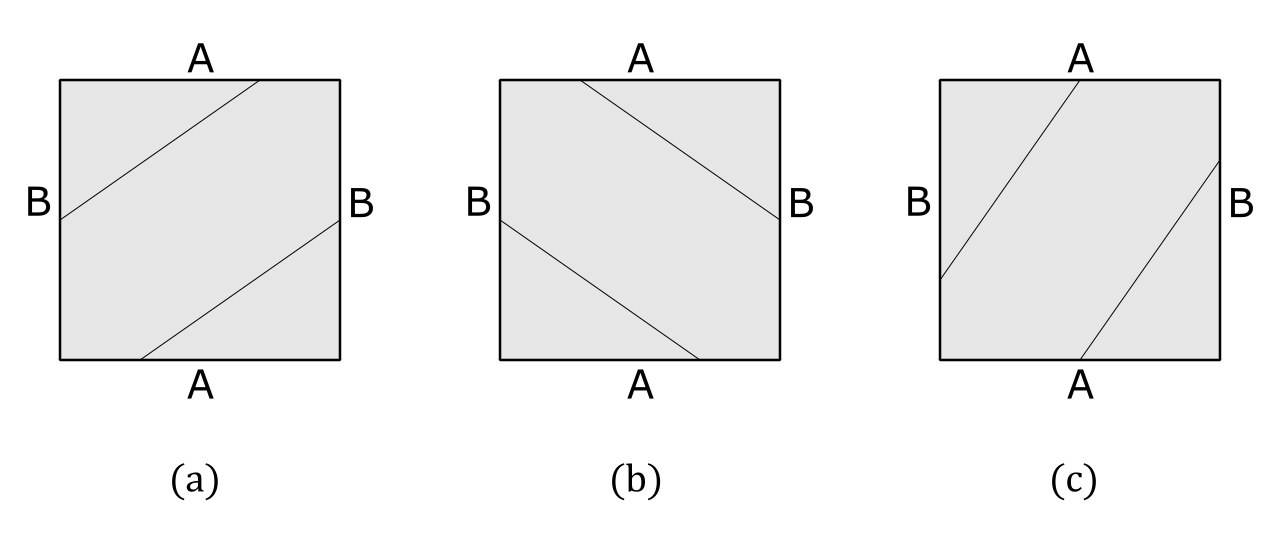
\includegraphics[scale=0.3]{2.5}
\caption{(a) Trajectory of slope 7/10 on the square torus (b) The result of a horizontal/vertical reflection (c) The result of a reflection along a diagonal}
\end{center}
\end{figure}

%Fig 2.6
\begin{figure} 
\begin{center}
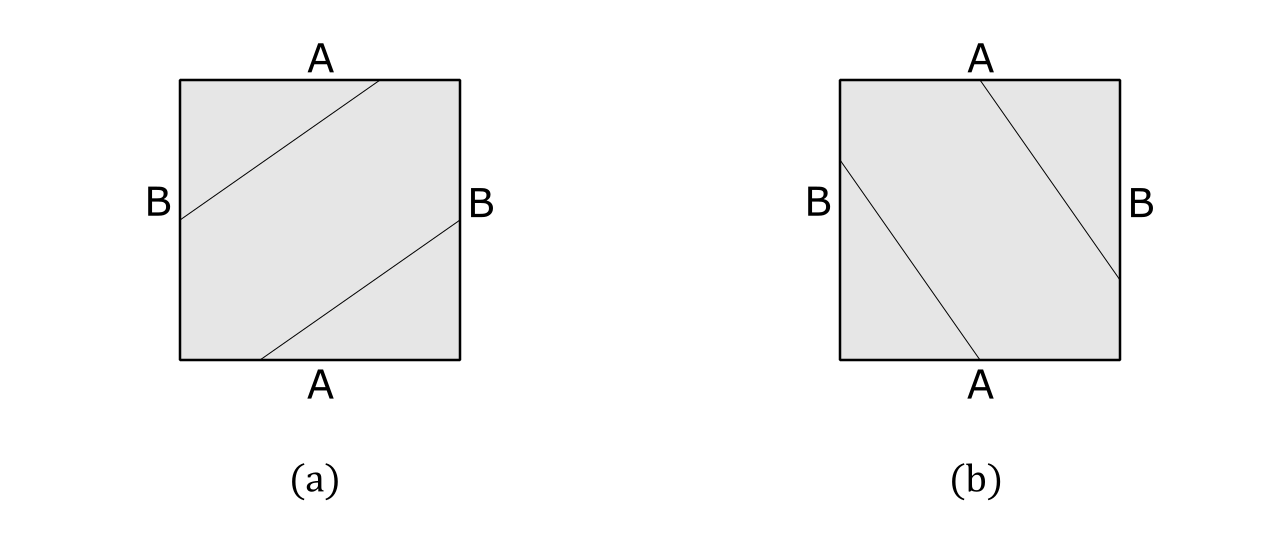
\includegraphics[scale=0.3]{2.6}
\caption{(a) Trajectory of slope 7/10 (b) The result of a $\pi/2$ clockwise or anti-clockwise rotation}
\end{center}
\end{figure}

 %Fig 2.7
\begin{figure} 
\begin{center}
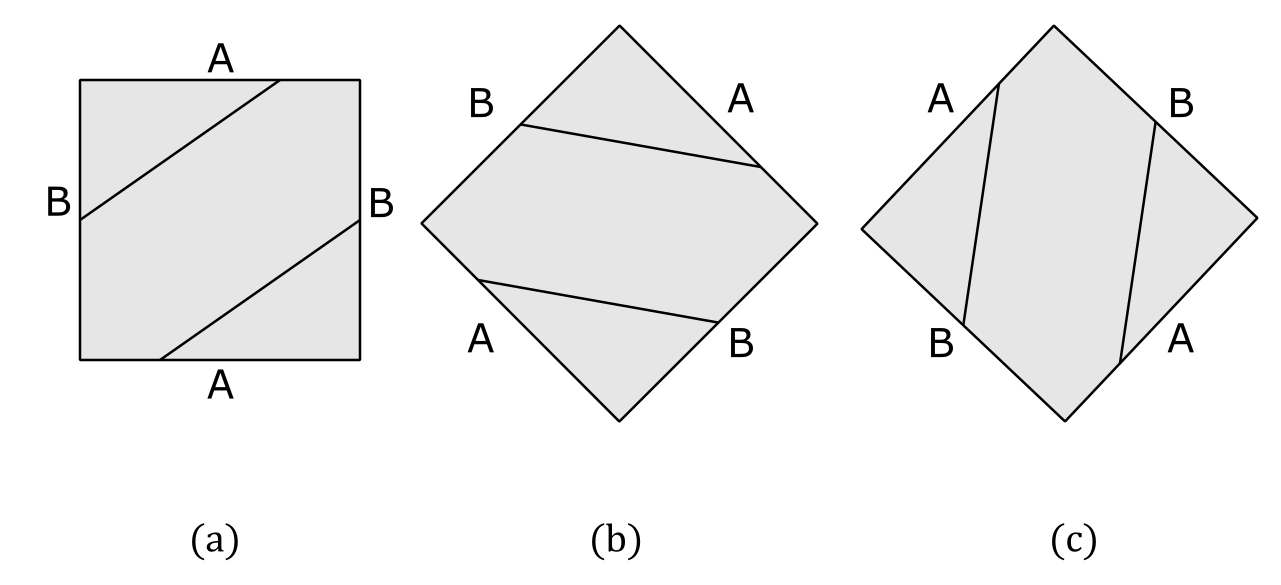
\includegraphics[scale=0.3]{2.7}
\caption{(a) Trajectory of slope 7/10 (b) The result of a $\pi/4$ clockwise rotation (c) The result of a $\pi/4$ anti-clockwise rotation}
\end{center}
\end{figure}


%Fig 2.8
\begin{figure} 
\begin{center}
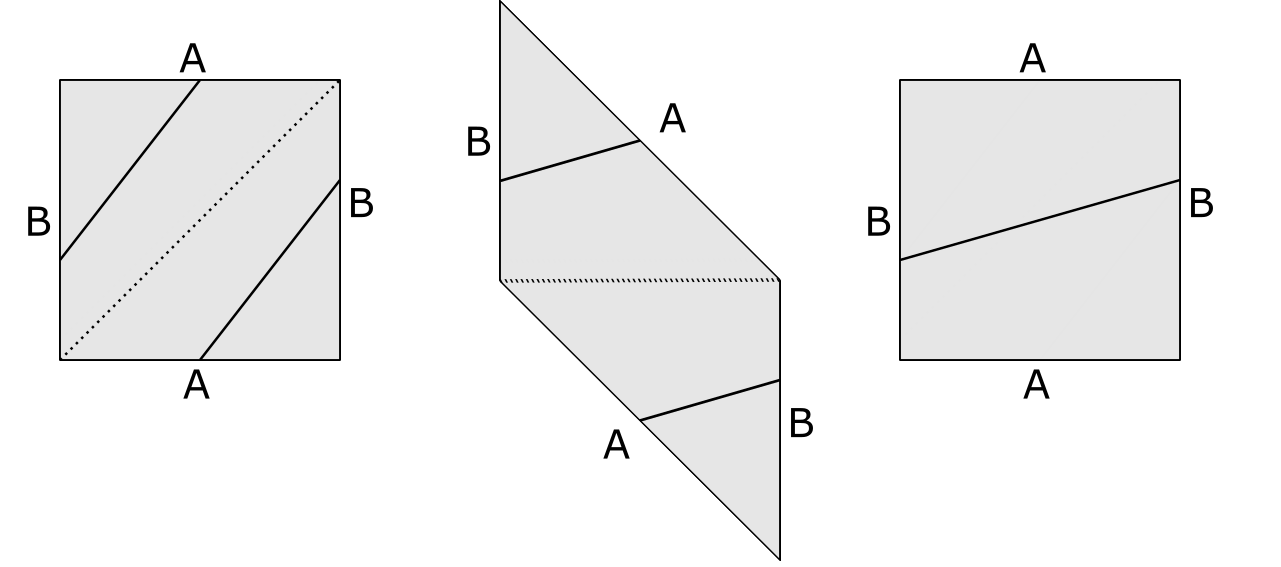
\includegraphics[scale=0.3]{2.8}
\caption{A square torus sheared and re-assembled (by translation) back into a square torus}
\end{center}
\end{figure}

\pagebreak

\section{Continued fractions}

\paragraph{Continued fractions are a method of representing real numbers in terms of a (finite or infinite) sequence of integers, using a general algorithm. \\ Eg- Continued fraction expansion of $\frac{13}{5}$ and $\pi$ (show the algorithm via these examples)}


\begin{displaymath}
{\frac{13}{5} = 2 + \frac{1}{\frac{13}{5}} = 2+ \frac{1}{1 + \frac{2}{3}} = 2+ \frac{1}{1 + \frac{1}{\frac{3}{2}}} = 2+ \frac{1}{1 + \frac{1}{1 + \frac{1}{2}}}}
\end{displaymath}

 
\paragraph{Thus, the continued fraction expansion of $\frac{13}{5}$ is $[2;1,1,2]$ \\ Above example resulted in finite expansion, the folowing expansion of $\pi$ shows that expansions can be never ending.}

\begin{displaymath}
{\pi = 3 + \frac{1}{7 + \frac{1}{15 + \frac{1}{1 + \frac{1}{292 + \frac{1}{1 + \frac{1}{1 + \frac{1}{\ddots}}}}}}}}
\end{displaymath}


\paragraph{Thus, the continued fraction expansion of $\pi$ is $[3; 7, 15, 1, 292, 1, 1,\cdots]$}


\begin{enumerate}

\item  {We started with the original number (say, $\sfrac{a}{b}$) in improper fraction form}
\item  {We subtracted an integer from it such that the remainder fraction is < 1}
\item  {The remainder fraction, we represent in terms of its reciprocal (Thus, if the remainder fraction is $\sfrac{p}{q}$, then we write it as $\sfrac{1}{\sfrac{q}{p}}$. Note that $\sfrac{q}{p}$ in this case is > 1}
\item  {We repeat the previous steps, with $\sfrac{q}{p}$ instead of $\sfrac{a}{b}$ in step 1.}
\item  {We carry this procedure out till the process cannot be continued anymore. (for a rational number, this will mean that a proper fraction with numerator = 1 has been obtained.)}
\end{enumerate}

\paragraph{Note that this algorithm relies on two key steps- subtracting an integer from an improper fraction, and taking the reciprocal of a proper fraction to turn into an improper fraction. We form the final expansion using the integers that we subtract in alternating steps.
\\
We introduce continued fractions because, as we shall see, there is a powerful relationship between cutting sequences of a trajectory, and the continued fraction expansion of its slope.}

\section{Analysis of Trajectories}

\paragraph{Having set up the tools of analysis of a square torus, we can begin to analyze trajectories on the square torus. 
\\ \\
We start by asking an important question regarding cutting sequences- which of them are valid? How can we be sure that a given permutation of $A$’s and $B$’s corresponds to a valid cutting sequence on the square torus? The following theorem will help us in figuring out which sequences are not valid.}

\begin{theorem}
$A$ cutting sequence featuring two consecutive $A$’s somewhere and also two consecutive $B$’s somewhere, is an invalid cutting sequence.
\end{theorem}

\begin{proof}
If a cutting sequence has AA’s somewhere then it passes through the diagonal, and it must have a slope greater than 1. \\ 
If a cutting sequence has BB’s somewhere, it also must pass through the diagonal, but its slope must be smaller than 1. \\ 
Since, a cutting sequence can only represent a single slope, it's not possible to have AA’s and BB’s somewhere in the same cutting sequence (Fig 2.9).
\end{proof}

%Fig 2.9
\begin{figure}[h] 
\begin{center}
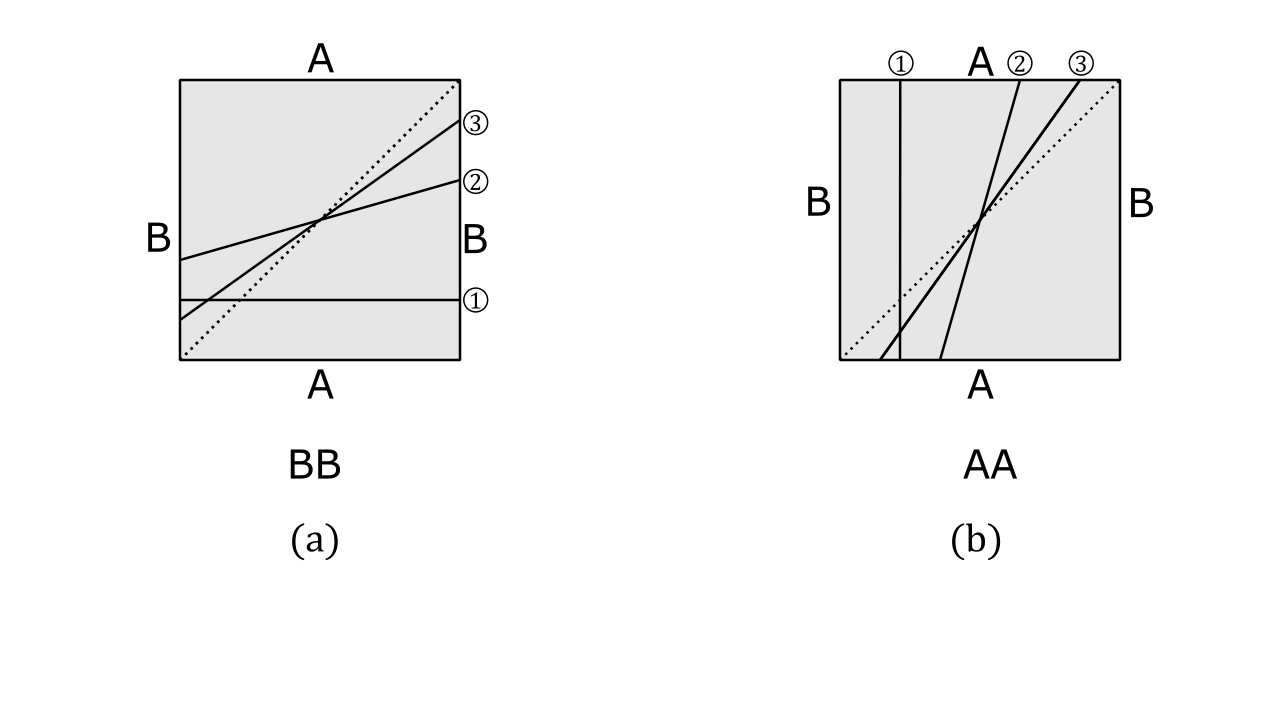
\includegraphics[scale=0.3]{2.9}
\caption{(a) Trajectory $\overline{BB}$ cutting the diagonal (b) Trajectory $\overline{AA}$ cutting the diagonal
}
\end{center}
\end{figure}

\begin{theorem}
A cutting sequence featuring both blocks of multiple A’s separated by single B’s and blocks of multiple B’s separated by single A’s, is an invalid cutting sequence.
\end{theorem}

\paragraph{We would like to use these conditions to obtain a list of all valid cutting sequences on the square torus. However, it is not feasible to try and characterize cutting sequences individually into groups of valid and invalid. Fortunately, we find that, using the symmetry transformations, we can create an algorithm to create new sequences from a given sequence. If the given sequence turns out to be invalid, it will render all the generated sequences invalid too.}

\paragraph{Consider a trajectory $\tau$ on the surface. If we apply a symmetry transformation \textit{T} on the square torus, it also acts on $\tau$ to give us a new trajectory $\tau^{'}$, with its own cutting sequence $c(\tau^{'})$. Thus, we may obtain a new (and valid) cutting sequence by applying \textit{T} to a given valid sequence  $c(\tau)$.}

\paragraph{The exact effects on cutting sequences after applying symmetries to the surface are as follows:}

\begin{enumerate}
\item  {\emph{Reflection:} If \textit{T} is the reflection transformation along horizontal or vertical lines of symmetry, we observe $c(\tau)$ and $c(\tau^{'})$ remain the same. If \textit{T} is reflection along a diagonal line of symmetry, $c(\tau^{'})$ is $c(\tau)$ with A’s replaced with B’s and B’s replaced with A’s.}
\item  {\emph{Rotation:}If \textit{T} is a rotation by an odd multiple of $\sfrac{\pi}{2}$, we observe $c(\tau)$ is $c(\tau^{'})$ with A’s replaced with B’s and B’s replaced with A’s. The cutting sequence remains unchanged (i.e. $c(\tau^{'})$ is $c(\tau)$) when \textit{T} is a rotation is made by an even integral multiple of $\sfrac{\pi}{2}$}
\item  {\emph{Shearing:}This one is not nearly as simple. We will consider a specific shear map as an example. \\
Let $M = \begin{bmatrix} 1&0\\-1&1 \end{bmatrix}$ This is a map that shears the square torus vertically downwards (Fig 2.10) }
\end{enumerate}

%Fig2.10
\begin{figure} 
\begin{center}
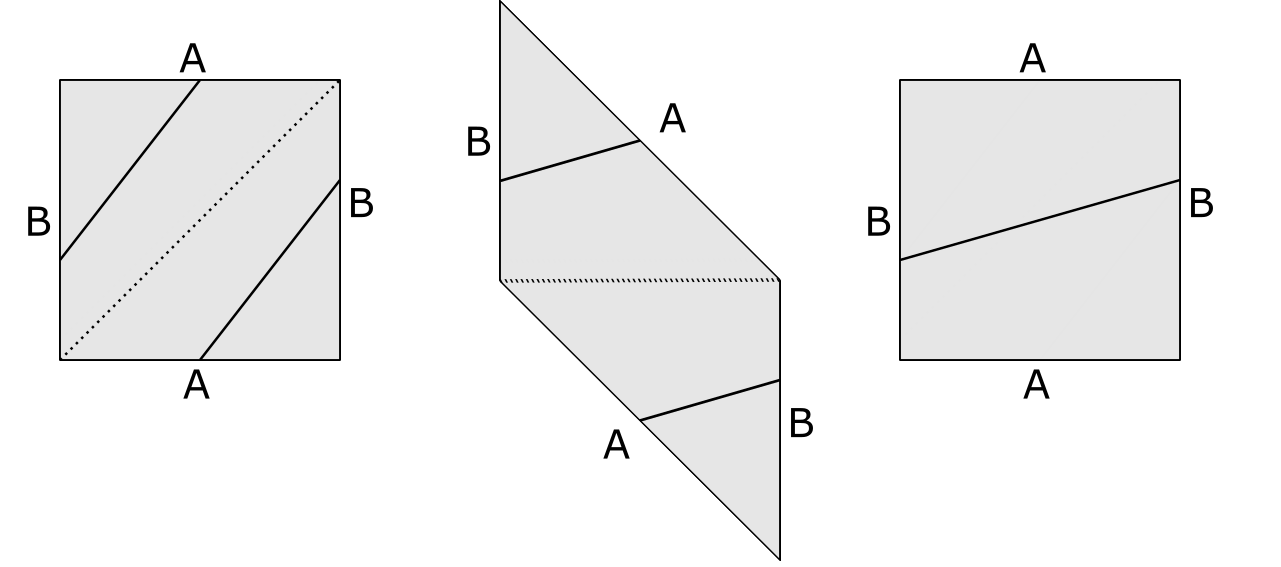
\includegraphics[scale=0.3]{2.10}
\caption{The action of a shearing transformation on a trajectory on the square torus}
\end{center}
\end{figure}

\paragraph{Consider a trajectory $\tau$ on the torus. We notice the following things about its cutting sequence $c(\tau)$:}
\begin{itemize}
\item  {Since the shearing map does not affect the square torus horizontally, we find that M makes no difference to the number of B’s in $c(\tau)$}
\item  {We see that the horizontal side A in the sheared square torus corresponds to the diagonal in the unsheared square torus. We also see that, for any trajectory with slope greater than 1 (i.e, 2 consecutive A’s in the cutting sequence) it must pass through the diagonal line of the unsheared square torus (Fig 2.10). Which means, for two consecutive A’s in the unsheared trajectory, we obtain one A in the sheared trajectory, and for a single A in the unsheared trajectory, we obtain no A in the sheared trajectory (since a single A means that that segment of $\tau$ goes from A to B, and thus, does not pass the diagonal)}
\end{itemize}

\paragraph{From these two observations, we infer that in going from $c(\tau)$ to $c(\tau ^{'})$, we keep the B’s unchanged, but we reduce the number of A’s in each set of A’s separated by B’s. }

\paragraph{Note- We know from Appendix-2 that }
$\begin{bmatrix} 1&0\\1&1 \end{bmatrix}^{n} = \begin{bmatrix} 1&0\\n&1 \end{bmatrix}$

\paragraph{This means that applying the general shear (call it $M_{n}$) has the same effect as applying $M$, n number of times. Thus, the cutting sequence obtained by applying $M_{n}$ to  is the same as that obtained by applying $M$ to n times. This means that $M_{n}$, acting on, will result in a cutting sequence with the same number of B’s, and with n A’s removed from each block of A’s in $c(\tau)$.}


\section{Cutting Sequences and Continued fractions}

\paragraph{We now introduce our most powerful relation, utilizing the idea of continued fractions mentioned earlier, and the effect of the symmetry transformations on cutting sequences.}

\paragraph{Consider a periodic trajectory $\tau$ on the square torus with a rational slope $m$. We will select two linear transformations- 
a vertical shear
$S=\begin{bmatrix}
1&0\\-1&1
\end{bmatrix}$
and flipping about a diagonal 
$F=\begin{bmatrix}
0&1\\1&0
\end{bmatrix}$.
Note the effect of these transformation on $m$: $S$ reduces $m$ by 1, and $F$ gives $\tau’$ the reciprocal of the slope of $\tau$}

\paragraph{We apply $S$ and $F$ using the following algorithm (We shall term it the \textit{$S/F$ algorithm} in this text)-}

\begin{itemize}
\item  {If $m>1$, we apply $S$ repeatedly till the resultant slope is less than $1$}

\item  {If $m<1$, we apply $F$, to turn it into a resultant slope that is greater than $1$}

\item  {If $m=0$, we stop.}
\end{itemize}

\paragraph{It is easy to see that there is a striking similarity between the process of applying $S$ and $F$, and the process of taking the continued fraction expansion of the slope of $\tau$. This similarity is what allows us to describe a process of converting a trajectory of a given slope into a horizontal trajectory (We will see why this is useful shortly)}

\paragraph{Let us solidify this relationship. Consider a periodic trajectory $\tau$  with slope $m$. Applying the $S/F$ algorithm to $\tau$ till the slope becomes $0$, gives us a series of steps (Applying $S$ a finite number of times, and applying $F$ once). Let $m_n$ be the slope after the nth step in the series. Applying the continued fraction algorithm to $m$ gives us the continued fraction expansion (another series of steps). Let $k_n$ be the fraction part left after the $nth$ step of the series. The following example explains what we mean by $k_n$ }

\begin{equation}
\frac{8}{5}=1+\frac{3}{5}=1+\frac{1}{\frac{5}{3}}=1+\frac{1}{1+\frac{2}{3}}=1+\frac{1}{1+\frac{1}{\frac{3}{2}}}=1+\frac{1}{1+\frac{1}{1+\frac{1}{2}}}
\end{equation}

\paragraph{(The highlighted number at the $nth$ step is $k_n$)}

\paragraph{We start by noting that at the $nth$ step, $m_n = k_n$ (as shown in fig) (note that this is the reason why we can be confident that the $S/F$ algorithm will eventually lead to $0$ slope, for a starting rational slope, since the fraction part of the continued fraction expansion for rational numbers will eventually become $0$)}

\paragraph{If the $n+1th$ step in the $S/F$ sequence involves $i$ consecutive $S$’s, then we subtract $i$ from $m_n$ so that $m_{n+1}$ is a proper fraction. In the continued fraction expansion, this $n+1th$ step will correspond to subtracting $i$ from $k_n$, so that $k_{n+1}$ is a proper fraction (This is because $m_n = k_n$). Note also that $i$ will be an entry in the final continued fraction expansion (since $k_n$ is written as $i + k_{n+1}$). \textit{Thus, a consecutive set of $i$ applications of $S (= S_i)$ to the trajectory corresponds to a continued fraction expansion entry of value $i$ -- (1)}}

\paragraph{If the $n+1th$ step in the $S/F$ sequence involves an $F$, then we take the reciprocal of $m_n$, so that $m_{n+1}$ is $\frac{1}{m_n}$ (note that since we are applying $F$, $m_n$ must be proper). In the continued fraction expansion, this $n+1th$ step will correspond to taking the reciprocal of $m_n$ (This is because, since $m_n = k_n$, $k_n$ is also proper, and so we take the reciprocal according to the continued fraction algorithm). Note that the next ($n+2th$) step in the continued fraction algorithm will add a new term to the expansion, and the $n+2th$ step in the $S/F$ algorithm is to apply $S$ (since $m_{n+1}$ is improper). \textit{Thus, each $F$ in the $S/F$ algorithm corresponds to a transition from one entry in the continued fraction algorithm, to the next entry.-- (2)}}

\paragraph{Thus, we see that there is a very elegant relationship between transformations using $S$ and $F$, and the continued fraction expansion of the slope of a trajectory. We see that we can use the continued fraction expansion of the slope to understand precisely how a trajectory has been transformed (using statements \textit{(1)} and \textit{(2)}). This is extremely useful for us, because it enables us to arrive at the exact cutting sequence of a trajectory, given only the slope.  (note that up till now, we have only known how to calculate the number of $A$’s and $B$’s in the sequence, given the trajectory slope. Now, we can know the exact sequence).}

\paragraph{The following theorem illustrates how we approach the process of obtaining a cutting sequence from the slope.}

\paragraph{\textit{THEOREM- Suppose a periodic trajectory $\tau$ on the square torus has a slope $m=\frac{p}{q}$. Let $[c_1, c_2,..., c_n]$ be the continued fraction expansion of $m$. Then, starting from the horizontal trajectory (given by the cutting sequence $\bar{B}$), we can use the continued fraction expansion of $m$ to obtain the exact cutting sequence of $\tau$ as follows:}}

\begin{enumerate}
\item  { \textit{Start with a string of B’s.}}

\item  { \textit{Add $c_n$ $A$’s between each consecutive pair of $B$’s}}

\item  { \textit{Swap the $A$’s and $B$’s}}

\item  { \textit{Repeat out steps $2$ and $3$ for $c_{n-1}$,... till $c_1$}}
\end{enumerate}

\paragraph{\textit{The resultant cutting sequence is the one corresponding to $\tau$ , i.e, c($\tau$)}}

\paragraph{\textit{Proof:}We chose $p+q$ $B$’s because we already know that is the period of the trajectory. We already know that the exact way in which we apply $S$ and $F$ tells us how the cutting sequence changes at each step (refer section on symmetries). Thus, we assume that $c(\tau)$ exists, and that a particular series of $S$ and $F$ transformations is applied to $\tau$ according to the $S/F$ algorithm. All we need to do then, is travel back along the series (essentially, undo the series, starting from the final $B$ sequence). We will arrive at $c(\tau)$.}

\paragraph{Since we know how to interpret the steps of the $S/F$ algorithm exactly in terms of the continued fraction expansion of $m$, we can simply carry out the undoing process in terms of the expansion. Since $c_i$ in the expansion corresponds to applying $S$ $c_i$ times (which in turn means we remove $c_i$ $A$’s from each consecutive set of $A$’s), in the undoing process we just add $c_i$ $A$’s between every consecutive pair of $B$’s to the sequence. Going from $c_i$ to $c_{i+1}$ corresponds to applying $F$ (which in turn means we swap the $A$’s and $B$’s), so in the undoing process we simply swap the $A$’s and $B$’s in moving from  $c_i$ to $c_{i+1}$.}

\paragraph{We illustrate this method using the following example:}


\paragraph{\textit{EXAMPLE:} We will find the cutting sequence of a trajectory $\tau$ with slope $m=\frac{5}{3}$. To do so, we first find the continued fraction expansion of $\frac{5}{3}$ }

\begin{equation}
\frac{5}{3}=1+\frac{2}{3}=1+\frac{1}{\frac{3}{2}}=1+\frac{1}{1+\frac{1}{2}}
\end{equation}

\paragraph{Thus, the continued fraction expansion of $\frac{5}{3}$ is $[1,1,2]$}

\begin{enumerate}
\item  {We start with a bi-infinite sequence of B’s.
\\* \\* $\overline{B}$}

\item  {Add 2 A’s to each collection of A’s, since the last entry in the continued fraction expansion is 2.
\\* \\* $\overline{BAA}$}

\item  {Flip the A’s and B’s
\\* \\* $\overline{ABB}$}

\item  {Add 1 A to each collection of A’s (since the 2nd entry in continued fraction expansion is 1).
\\* \\* $\overline{AABAB}$}

\item  {Flip the A’s and B’s
\\* \\* $\overline{BBABA}$}

\item  {Add 1 A to each collection of A’s (since the 2nd entry in continued fraction expansion is 1)
\\* \\* $\overline{BABAABAA}$}
\end{enumerate}

\paragraph{Thus, $\overline{BABAABAA}$ is the continued fraction expansion of a trajectory of slope $\frac{5}{3}$ on the square table.}


\paragraph{Note- We have, in our entire analysis, considered trajectories with slope in the range $[0, \pi/2]$. However, we may extend all our discussions to the $[$-$\pi/2, 0]$ range by simply observing that if a cutting sequence corresponds to a particular slope $m$, then the exact same cutting sequence corresponds to -$m$. This is because a trajectory of slope -$m$ can be created by flipping the table containing a trajectory with slope $m$ (i.e, an orientation reversing vertical flip). Since this preserves the positions of side $A$ and $B$ in the square torus, the cutting sequence remains unchanged. Thus, a trajectory of slope -$m$ has the same cutting sequence that a trajectory of slope $m$ does.}



\appendix

\chapter{Properties regarding vertices on a surface}

\section{Flat surfaces}

\paragraph{To test whether a surface is flat, we do two simple tests:}

\begin{itemize}
\item  {The given surface is kept on a plane table, if the surface is plane, we won’t see any peaks or trenches. The given surface sticks to the plane table.}

\item  { We measure the angle around the vertices (the points along which the surface can be rolled and twisted). If the angle comes out to be an integral multiple of $2\pi$, we can say that surface is flat.}
\end{itemize}

\paragraph{These two tests leave us with the following definition of a plane surface.}



\paragraph{\textit{DEFINITION}: A surface is called flat if it looks like the flat plane everywhere, except possibly at finitely many cone points (vertices), where the vertex angle is a multiple of $2\pi$.}

\paragraph{Test 1 is an observation. We can mentally or physically see if kept on a plane surface, do we see a plane surface or a surface with ups and downs.}

\paragraph{Test 2 is a calculation. We must know the process to determine an angle around a vertex.}

\paragraph{To measure the angle around a vertex we use the following step sequence:}

\begin{enumerate}
\item  {Identify all the vertices (as given in section 1.3}

\item  {Select any vertex and select its opposite identified point.}

\item  {Draw an arrow in the anti-clockwise direction between the edges that contain that point.}

\item  {Find the oppositely identified edge, of the edge that touches the head of arrow.}

\item  {From the edge identified in step 4, we draw another arrow that goes in the same direction as given by the arrow in step 3.}

\item  {Repeat steps 4 and 5 until we reach the initially selected point and the whole surface vertex is surrounded.}

\item  {Now measure angles of the identified polygon vertices, and add them up. This is the angle around the surface vertex in question}
\end{enumerate}


\section{Vertices of a Regular 2n-gon}

\paragraph{We state and prove a theorem regarding the number of vertices of a surface made by identifying a regular 2n-gon (a polygon with 2 sides)}

\paragraph{\textit{THEOREM}- If $S_G$ is a surface made by identifying the oppositely oriented edges of a $2n$-gon $G$, then 
$S_G$ has 2 vertices if $n$ is odd, and 1 vertex if $n$ is even}

\paragraph{\textit{Proof}:We take a $2n$-gon $G$, and identify it into a surface $S_G$. Let $G$ have vertices $V_1$, $V_2$,....$V_2n$}

\paragraph{Consider the vertex identification process in section 1.3}

\paragraph{Notice that in this process, we start with a vertex each from side 1 and 1’ (say, $V_1$ and $V_1’ = V_k$), and then start identifying alternating vertices, proceeding clockwise or anticlockwise from $V_1$ and $V_1’$. It is clear that all vertices of an even index will be definitely identified together (same for odd indexed vertices) -- (1).}

\paragraph{The question is whether the odd vertices can be identified with even vertices.}

\paragraph{If $n$ is even, then $V_k$ has an even index ($k$ = even). This means that $V_1$ (an odd indexed vertex) and $V_k$ (an even indexed vertex) are identified. From statement (1) then, this means that all vertices are identified into 1 surface vertex in $S_G$.}

\paragraph{If $n$ is odd, then $V_k$ has an odd index ($k$ = odd). Since $V_1$ and $V_k$ are identified, the iteration of the identification process starting from $V_1$ will only include odd indexed vertices (since both $V_1$ and $V_k$ are odd indexed). Thus, we will need another iteration to identify all the even indexed vertices together, which means that we will have two surface vertices in $S_G$ in total.}



\chapter{All shears can be constructed from basic shears}

\paragraph{We will consider all integer shears here, i.e, shears of the form 
$\begin{bmatrix}
1&m\\0&1
\end{bmatrix}$
and
$\begin{bmatrix}
1&0\\n&1
\end{bmatrix}$,
where m and n are integers
We wish to prove that all such one directional shears can be created from 2 basic shears}


\paragraph{The basic shear maps are 
$\begin{bmatrix}
1&1\\0&1
\end{bmatrix}$
and
$\begin{bmatrix}
1&0\\1&1
\end{bmatrix}$
}

\paragraph{These maps have the following effect:}

\begin{enumerate}
\item  {The matrix
$\begin{bmatrix}
1&1\\0&1
\end{bmatrix}$
shears the square torus 
horizontally by unit length.
}

\item  {The matrix
$\begin{bmatrix}
1&0\\1&1
\end{bmatrix}$
shears the square torus vertically 
by unit length.
}
\end{enumerate}

\paragraph{Note that these are unit shears in the positive $x$ and $y$ directions. The inverse of these matrices will shear the square torus in the negative $x$ and $y$ directions respectively.}

\paragraph{We will now show that a general integer shear along the positive $y$ axis can be built using the unit shear in the same direction.}

\paragraph{\textit{THEOREM}- The general vertical shear map
$\begin{bmatrix}
1&0\\n&1
\end{bmatrix}$
can be written as
$\begin{bmatrix}
1&0\\1&1
\end{bmatrix}^n$,
where m is a positive integer
}

\paragraph{\textit{Proof}- We will prove this by induction. Note that}

\begin{equation}
\begin{bmatrix}
1&0\\1&1
\end{bmatrix}
\begin{bmatrix}
1&0\\1&1
\end{bmatrix}=
\begin{bmatrix}
1&0\\2&1
\end{bmatrix}
\end{equation}

\paragraph{Thus, the theorem holds for $n=1$ and $2$}

\paragraph{Now suppose it holds for $n=k$, i.e,}

\begin{equation}
\begin{bmatrix}
1&0\\1&1
\end{bmatrix}^k
=
\begin{bmatrix}
1&0\\k&1
\end{bmatrix}
\end{equation}

\paragraph{Then,}

\begin{equation}
\begin{bmatrix}
1&0\\1&1
\end{bmatrix}^{k+1}
=
\begin{bmatrix}
1&0\\k&1
\end{bmatrix}
\begin{bmatrix}
1&0\\1&1
\end{bmatrix}
=
\begin{bmatrix}
1&0\\k+1&1
\end{bmatrix}
\end{equation}

\paragraph{Thus, by induction, the theorem holds for all positive integer values of n}

\paragraph{For the negative integers, we note that the matrix for a unit shear in the negative $y$ direction is 
$\begin{bmatrix}
1&0\\-1&1
\end{bmatrix}$
(inverse of the positive unit vertical shear) The $nth$ power of this matrix can be shown to be 
$\begin{bmatrix}
1&0\\-n&1
\end{bmatrix}$
In that case, if n is a positive integer}

\begin{equation}
\begin{bmatrix}
1&0\\1&1
\end{bmatrix}^{-n}
=
\begin{bmatrix}
1&0\\-1&1
\end{bmatrix}^n
=
\begin{bmatrix}
1&0\\-n&1
\end{bmatrix}
\end{equation}

\paragraph{Thus, the theorem holds for negative integer values of $n$ too.}

\paragraph{A similar argument shows that
$\begin{bmatrix}
1&1\\0&1
\end{bmatrix}^m
=
\begin{bmatrix}
1&m\\0&1
\end{bmatrix}
$ 
for all integer $m$, giving us a general formula for all integer shears along the x axis.
}


\chapter{Drawing a given trajectory of $\frac{p}{q}$ slope on square torus.}


\paragraph{The basic rule we will exploit throughout the process is}

\begin{displaymath}
slope=\frac{\# of As}{\# of Bs}
\end{displaymath}

\paragraph{The above relation implies: The trajectory of slope $p/q$ intersects edge A $p$ times and edge B q times.}

\paragraph{Since the trajectory is a straight line, the points where the trajectory intersects with edges, must be equally spaced.}

\paragraph{We utilise following steps to draw any given trajectory of slope $\frac{p}{q}$ on the square torus:}

\paragraph{1. If p is odd}

\begin{enumerate}
\item[a]  {Make a mark on the midpoint of edge A}

\item[b]  {Now distribute the remaining $(p-1)$ points on either side of the midpoint, keeping them equally spaced from each other}
\end{enumerate}

\paragraph{\quad If $p$ is even}
\begin{enumerate}
\item[a]  {distribute the $p$ points on edge A, and ensure equal spaces between every consecutive point.}
\end{enumerate}

\paragraph{Note: Since in the square torus, the side B is really a circle, make sure the distance between extreme marked points is equal to all other spaces. Another way to look at it is to place extreme points at d/2 distance from the corner of the square, where d is the space between two consecutive points. Now, when we go between the extreme points via the vertex we find distance = d/2 + d/2 = d, the required distance. (Fig A.1)}

%Fig A.1
\begin{figure} 
\begin{center}
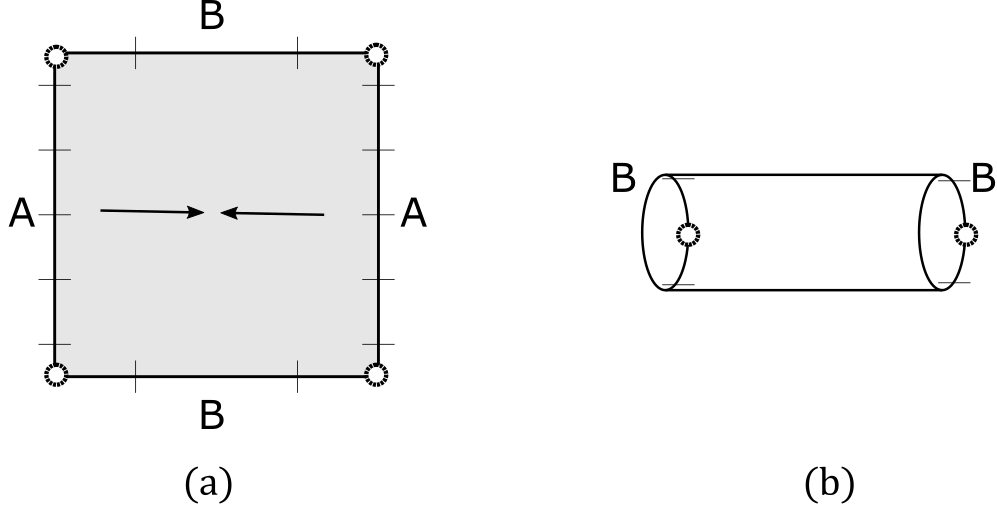
\includegraphics[scale=0.3]{a.1}
\caption{(a) Marks for a trajectory of slope 2/5 or -2/5 , (b) trajectory of slope 2/5 , (c) trajectory -2/5}
\end{center}
\end{figure}

\begin{enumerate}
\item[3]  {Repeat step 1 with $q$ on edge B}

\item[4]  {To join these points, we start at the top left vertex, go anti-clockwise for the points on the left and bottom edge, and clockwise for the sides top and right edge. We join corresponding indexed points (i.e, the first point going clockwise from the top left vertex to the first point going anti-clockwise, and so forth) (Fig A.2)}
\end{enumerate}

%Fig A.2
\begin{center}
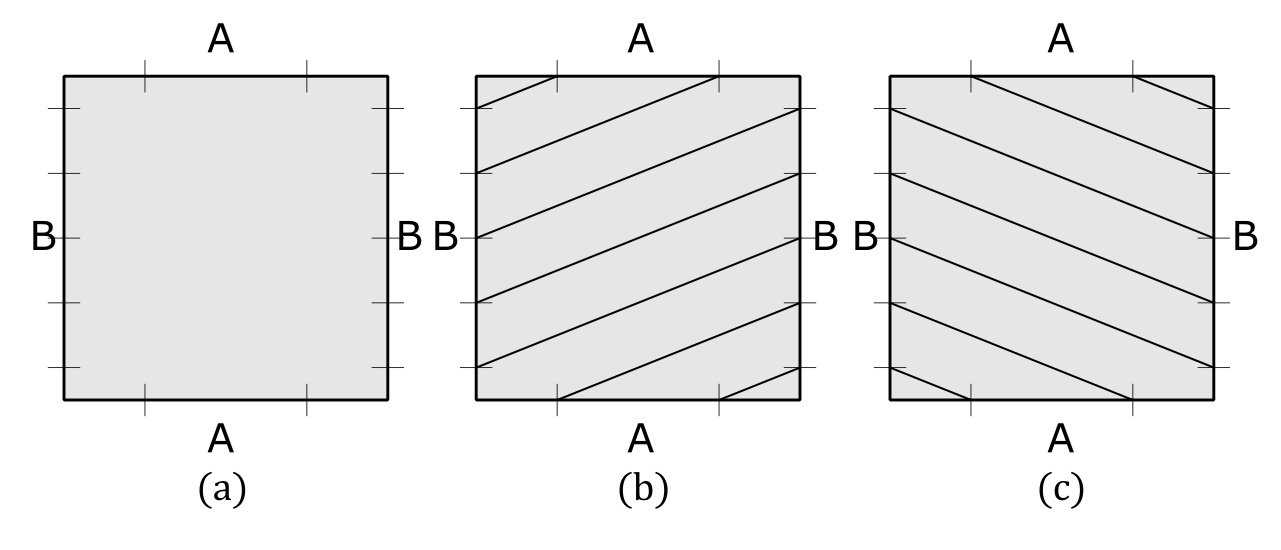
\includegraphics[scale=0.3]{a.2}
\end{center}

\paragraph{We can thus successfully draw a trajectory of slope p/q on the square torus using cutting sequences.}


\end{document}
